\documentclass[10pt]{beamer}

\usetheme{metropolis}
\usepackage{appendixnumberbeamer}

\usepackage{booktabs}
\usepackage[scale=2]{ccicons}
\usepackage{graphicx}
\usepackage{pgfplots}
\usepgfplotslibrary{dateplot}
\usepackage{caption}
\usepackage{subcaption}
\usepackage{xspace}
\usepackage{hyperref,xcolor}
\usepackage{textpos}

\usepackage{makeidx}
\definecolor{winered}{rgb}{0.5,0,0}
\newcommand{\themename}{\textbf{\textsc{metropolis}}\xspace}


\defbeamertemplate*{background canvas}{bg}
{%
	\color{white}\vrule width\paperwidth height\paperheight% added bg color
}





\title{Bhabha Tracking Efficiencies}
%\subtitle{A modern beamer theme}
\date{12.04.2019}
\author{Martin Sobotzik}
\institute{Johannes Gutenberg Universit\"at Mainz}
% \titlegraphic{\hfill
\includegraphics[height=1.5cm]{logo.pdf}}

\definecolor{darkblue}{rgb}{0,0,.5}
\hypersetup{pdftex=true, colorlinks=true, breaklinks=true, linkcolor=darkblue, menucolor=darkblue, pagecolor=darkblue, urlcolor=darkblue}


%citecolor={winered} %Gives errors when turned on
%allcolors={winered} %Gives errors when turned on

\begin{document}

\maketitle
{%
\setbeamertemplate{frame footer}{Bhabha Tracking Efficiencies}

%\section{Reproducing Plots}


\begin{frame}{Motivation}

\begin{itemize}	
	\item I am performing an analysis to estimate the tracking efficiency on phase 2 data
	\item The physics case I am considering is Bhabha events $\textrm{e}^+ \textrm{+e}^- \rightarrow \textrm{e}^+ \textrm{+e}^- $ 
	\item The definition of efficiency I am going to use is:

\end{itemize}
	\begin{equation*}
		\epsilon = \frac{\textrm{Number of Bhabha events with exactly 2 tracks}}{\textrm{Number of Bhabha events with 1 or more tracks}}
	\end{equation*}
	
	\begin{itemize}
		\item After selecting Bhabha events where at least one of the tracks was detected, one can look how many times the second one is found
		\item  This idea comes from some plots presented by Sam Cunliffe in previous  \href{https://confluence.desy.de/display/BI/ECL+Meetings?preview=/84320165/109161400/SCunliffe181123-ECL.pdf}{tracking and ECL} meetings.
	\end{itemize}





\end{frame}
	
	
	\begin{frame}{Motivation}
		\begin{figure}
			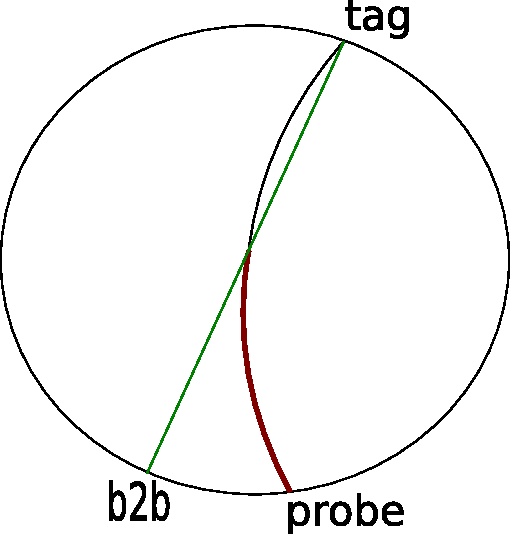
\includegraphics[width=5cm]{Plots/b2b}
		\end{figure}
	\end{frame}
	
	
	
	
\begin{frame}{Motivation}
	\begin{textblock*}{0.5\textwidth}(5cm,-3cm)
		

	
	
	\begin{itemize}
		
		\item $\textrm{gamma:probe}$ '$(\textrm{E} > 0.1 )$'
		\item $\textrm{gamma:tag}$ '$(\textrm{clusterE} > 3.0)$'

			\item $0.296706 < \theta < 2.61799 \rightarrow$ It has to hit the ECL
			\item $\textrm{nCleanedTracks}[ \textrm{abs}(\textrm{dz}) < 2.0 \textrm{ and } \textrm{abs}(\textrm{dr}) < 0.5 \textrm{ and nCDCHits} > 0 \textrm{ and pt } > 0.15] < 1 \rightarrow $ bad quality hits 
						
		\end{itemize}

	\end{textblock*}

	
\begin{textblock*}{0.5\textwidth}(0cm,-2.5cm)
	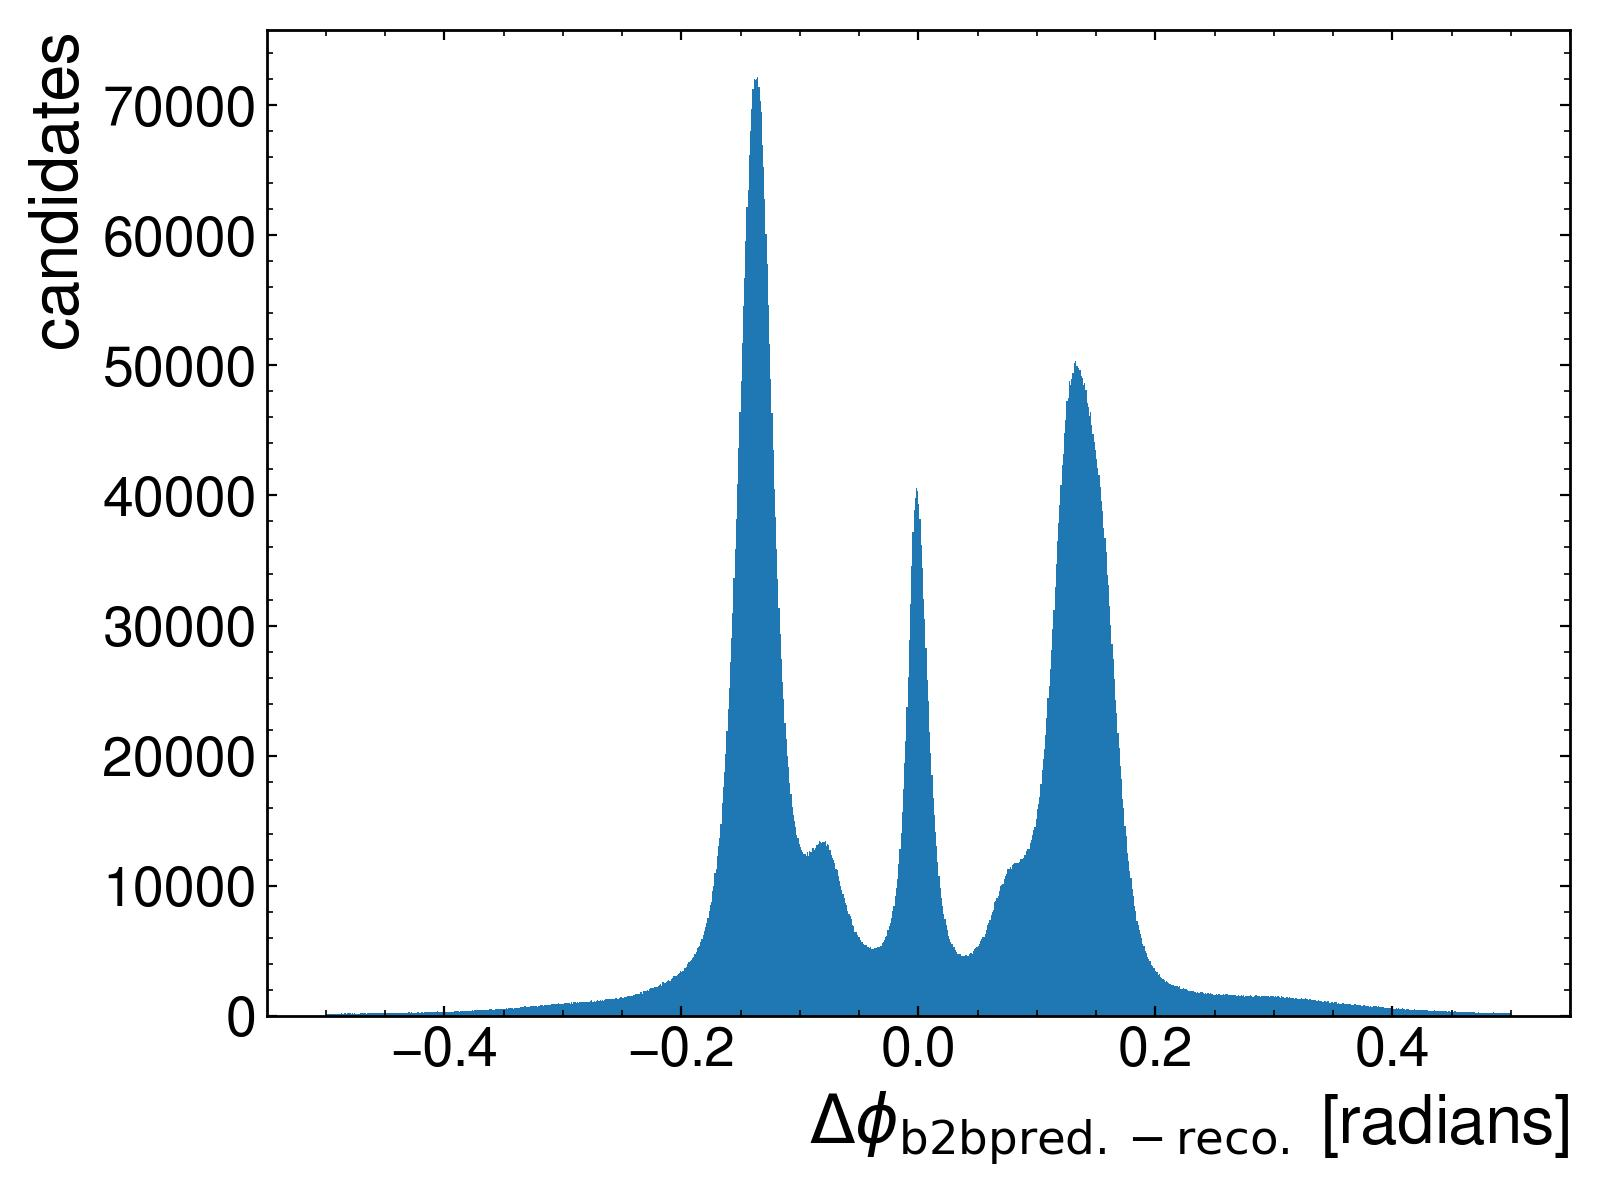
\includegraphics[width=4.5cm]{Plots/deltaPhiSam}
\end{textblock*}

\begin{textblock*}{0.5\textwidth}(-0.3cm,1cm)
	$\textrm{vpho} \rightarrow \textrm{gamma:probe} + \textrm{gamma:tag}$
\end{textblock*}
	
\end{frame}

\begin{frame}{A first attempt}
	\begin{textblock*}{\textwidth}(0cm,-4cm)
	

\begin{itemize}
	\item Fill a list of all the particles with an ECL Cluster associated (gamma)
	\item Reconstruct a Bhabha event from 2 of these objects
	\item Select a proper region in the $\Delta \Phi$ plot and check how many times a track was associated to a cluster
	
\end{itemize}

\begin{figure}
	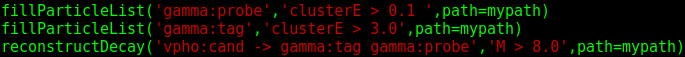
\includegraphics[width=10.5cm]{Plots/oldSc}
\end{figure}

	\end{textblock*}


	

	
	\begin{textblock*}{0.55\textwidth}(0.0cm,-0.2cm)
		\begin{figure}
			\includegraphics<1>[width=4.5cm]{Plots/DeltaPhi}
			\includegraphics<2>[width=4.5cm]{Plots/dphiMC}
		\end{figure}
	\end{textblock*}


		\begin{textblock*}{0.4\textwidth}(5.1cm,0.5cm)
			\begin{itemize}
				\item<1> Prod 6
		 \item<1> /hsm/belle2/bdata /Data/release-02-01-00 /DB00000438/prod00000006 /e0003/4S/r02*/all/mdst.sub00 /*.root
\end{itemize}
	\end{textblock*}
	
		\begin{textblock*}{0.55\textwidth}(5.1cm,-0.3cm)
	\begin{itemize}
		\item<2> MC11 $\textrm{ee}\rightarrow \textrm{ee}$
		\item<2> very few vpho reconstructed, no tracks associated to the daughters
		\item<2> $\rightarrow$ in the framework the gamma list is filled with objects with an ECL cluster and \underline{NO} track associated
		\item<2> $\rightarrow$ wrong object to use for our purposes
	\end{itemize}
\end{textblock*}



\begin{textblock*}{0.4\textwidth}(1cm,0cm)
	\only<1>{Plot on data:}
	\only<2>{Plot on MC:}
\end{textblock*}
	
	
\end{frame}




\begin{frame}{Learning from experience}
	\begin{textblock*}{\textwidth}(0cm,-4cm)
	
		\begin{itemize}
			
		\item To have a complete list of objects with an ECL cluster associated, one needs to "mix" two different lists, one of gammas and one of electrons
	
	\end{itemize}
	
\end{textblock*}
	\begin{textblock*}{\textwidth}(0cm,-2.9cm)
		
	
	\begin{figure}
		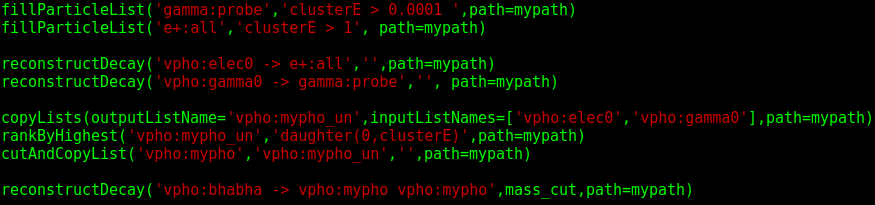
\includegraphics[width=10.5cm]{Plots/newSc}
	\end{figure}

\end{textblock*}
	
	
	\begin{textblock*}{\textwidth}(0cm,-0.3cm)
		

	\begin{itemize}
	\item The electron list does not require a ECL cluster$\rightarrow$ problem solved with the cut on clusterE
	\item The framework does not allow to mix lists of different types $\rightarrow$ problem solved with the "trick" of two intermediate virtual photons
	\item The ranking is a way for me to have the order of the daughters' under control
	\item The Bhabha candidates are finally reconstructed starting from 2 ECLobjects
\end{itemize}
	\end{textblock*}
\end{frame}



\begin{frame}{$\Delta \Phi$ distribution, Prodx6}


\begin{textblock*}{0.5\textwidth}(0cm,-2.5cm)
	\includegraphics<1>[width=5cm]{Plots/DataLeft}
	\includegraphics<2>[width=5cm]{Plots/DataAll}
\end{textblock*}

\begin{textblock*}{0.5\textwidth}(5cm,-3cm)
	\begin{itemize}
		\item Plot of $\Delta \Phi$ using the final vpho list
		\item \textcolor{blue}{daughter\_0\_b2bClusterPhi - daughter\_1\_clusterPhi}
		\item<2> \textcolor{red}{daughter\_1\_b2bClusterPhi - daughter\_0\_clusterPhi}
		\item<2> \textcolor{orange}{Added both hists}
	\end{itemize}
\end{textblock*}

	\begin{textblock*}{\textwidth}(0cm,1.5cm)
	\begin{itemize}
		\item<2> After adding the 2 hists I (of course) have double counted the events
		\item<2> For my studies it would make more sense to concentrate on only one side to avoid double counting
	\end{itemize}
\end{textblock*}



\end{frame}

\begin{frame}{$\Delta \Phi$ distribution, MC11}
	
	
	\begin{textblock*}{0.5\textwidth}(0cm,-2.5cm)
		\includegraphics<1>[width=5cm]{Plots/MCDPhi}
		
	\end{textblock*}
	
	\begin{textblock*}{0.5\textwidth}(5cm,-3cm)
		\begin{itemize}
			\item Plot of $\Delta \Phi$ using the final vpho list
			\item \textcolor{blue}{daughter\_0\_b2bClusterPhi - daughter\_1\_clusterPhi Reconstructed}
			\item \colorbox{blue}{\textcolor{white}{MCTruthMatched}}
			\item  \textcolor{red}{daughter\_1\_b2bClusterPhi - daughter\_0\_clusterPhi Reconstructed}
			\item \colorbox{red}{\textcolor{white}{MCTruthMatched}}
		
		\end{itemize}
	\end{textblock*}
	
	\begin{textblock*}{\textwidth}(0cm,2.5cm)
	\begin{itemize}
		\item The difference between reconstructed and MCTruthMatched is caused by inefficiency
		
	\end{itemize}
\end{textblock*}
	
\end{frame}




	

\begin{frame}{$\Delta \Phi$ distribution, MC}
	
	\begin{textblock*}{\textwidth}(0cm,-3.8cm)
		\begin{figure}
			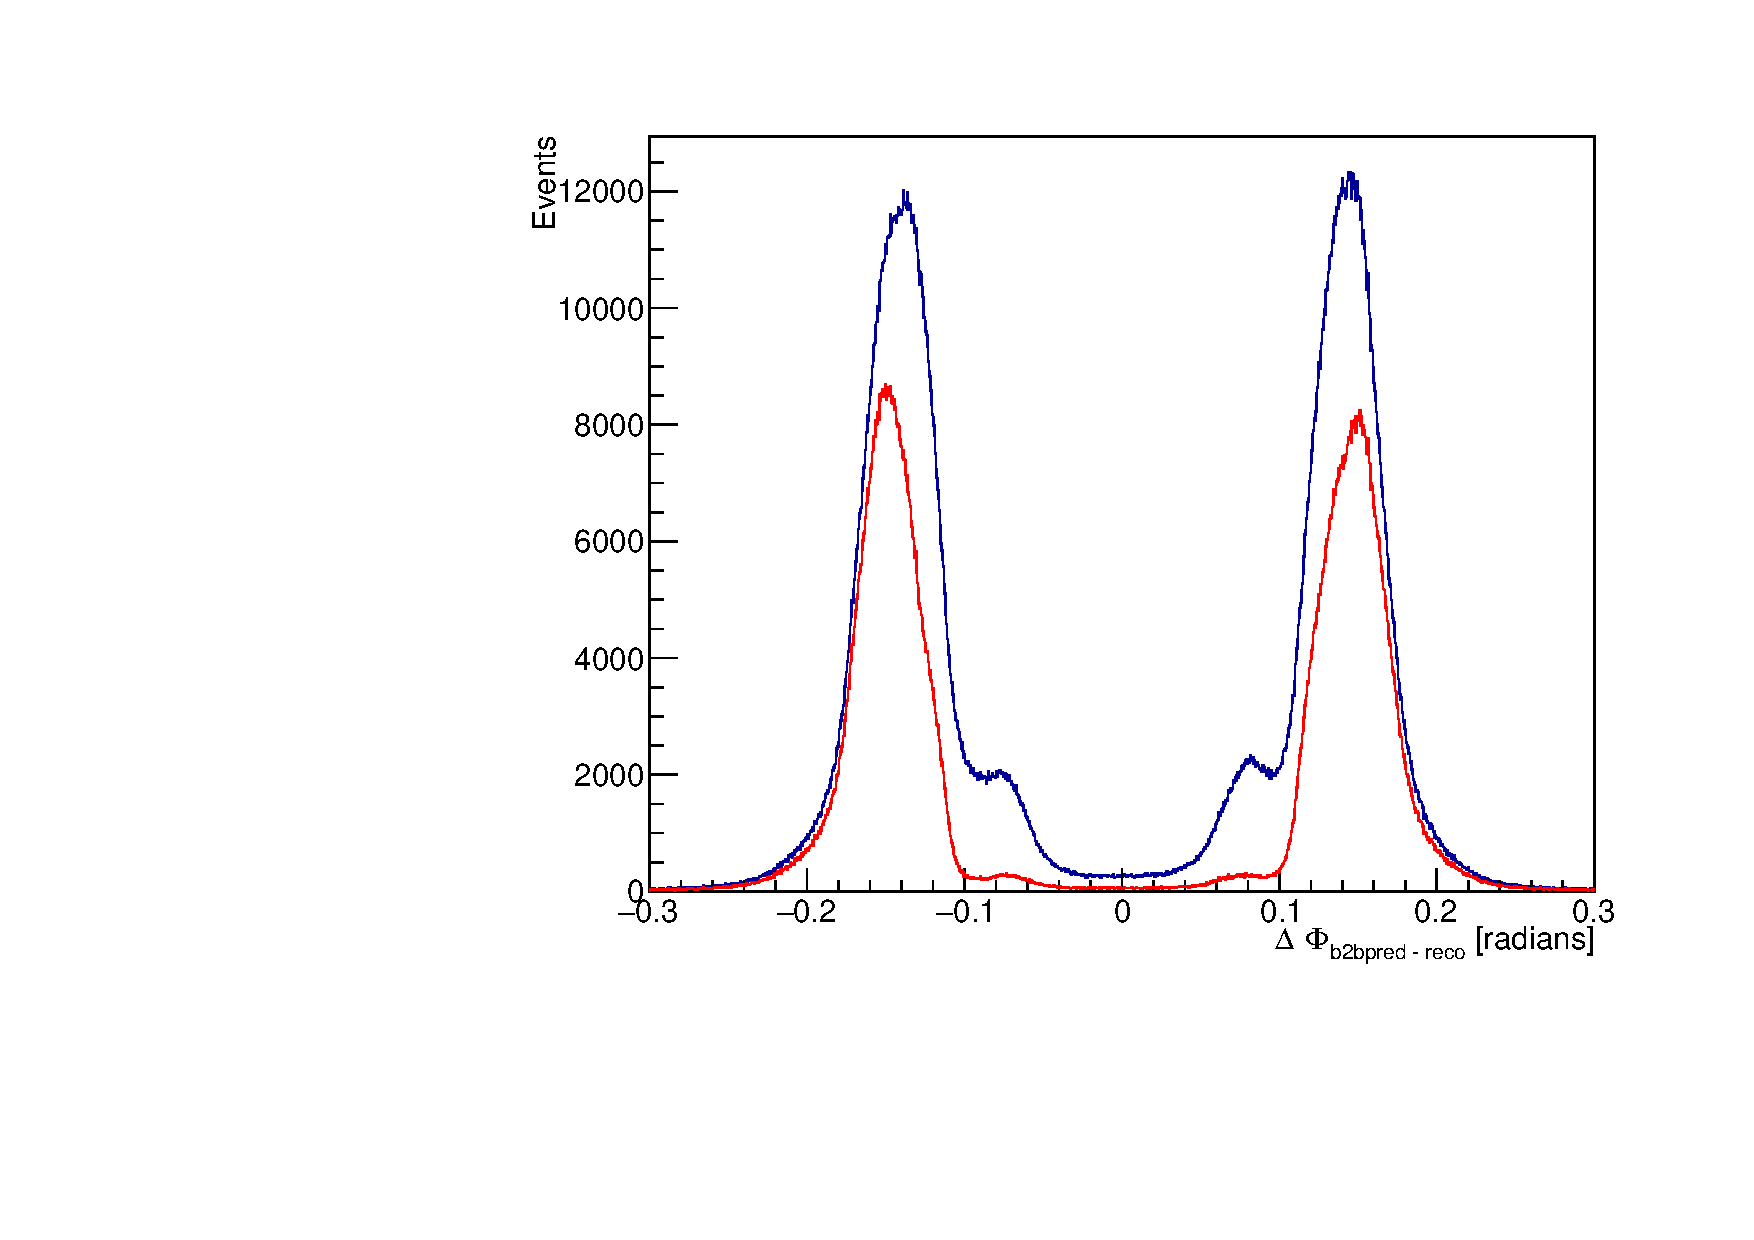
\includegraphics[width=4cm]{Plots/isSignalDeltaPhi}
		
		\end{figure}
	\end{textblock*}

\begin{textblock*}{\textwidth}(-4cm,-0.5cm)
	\begin{figure}
		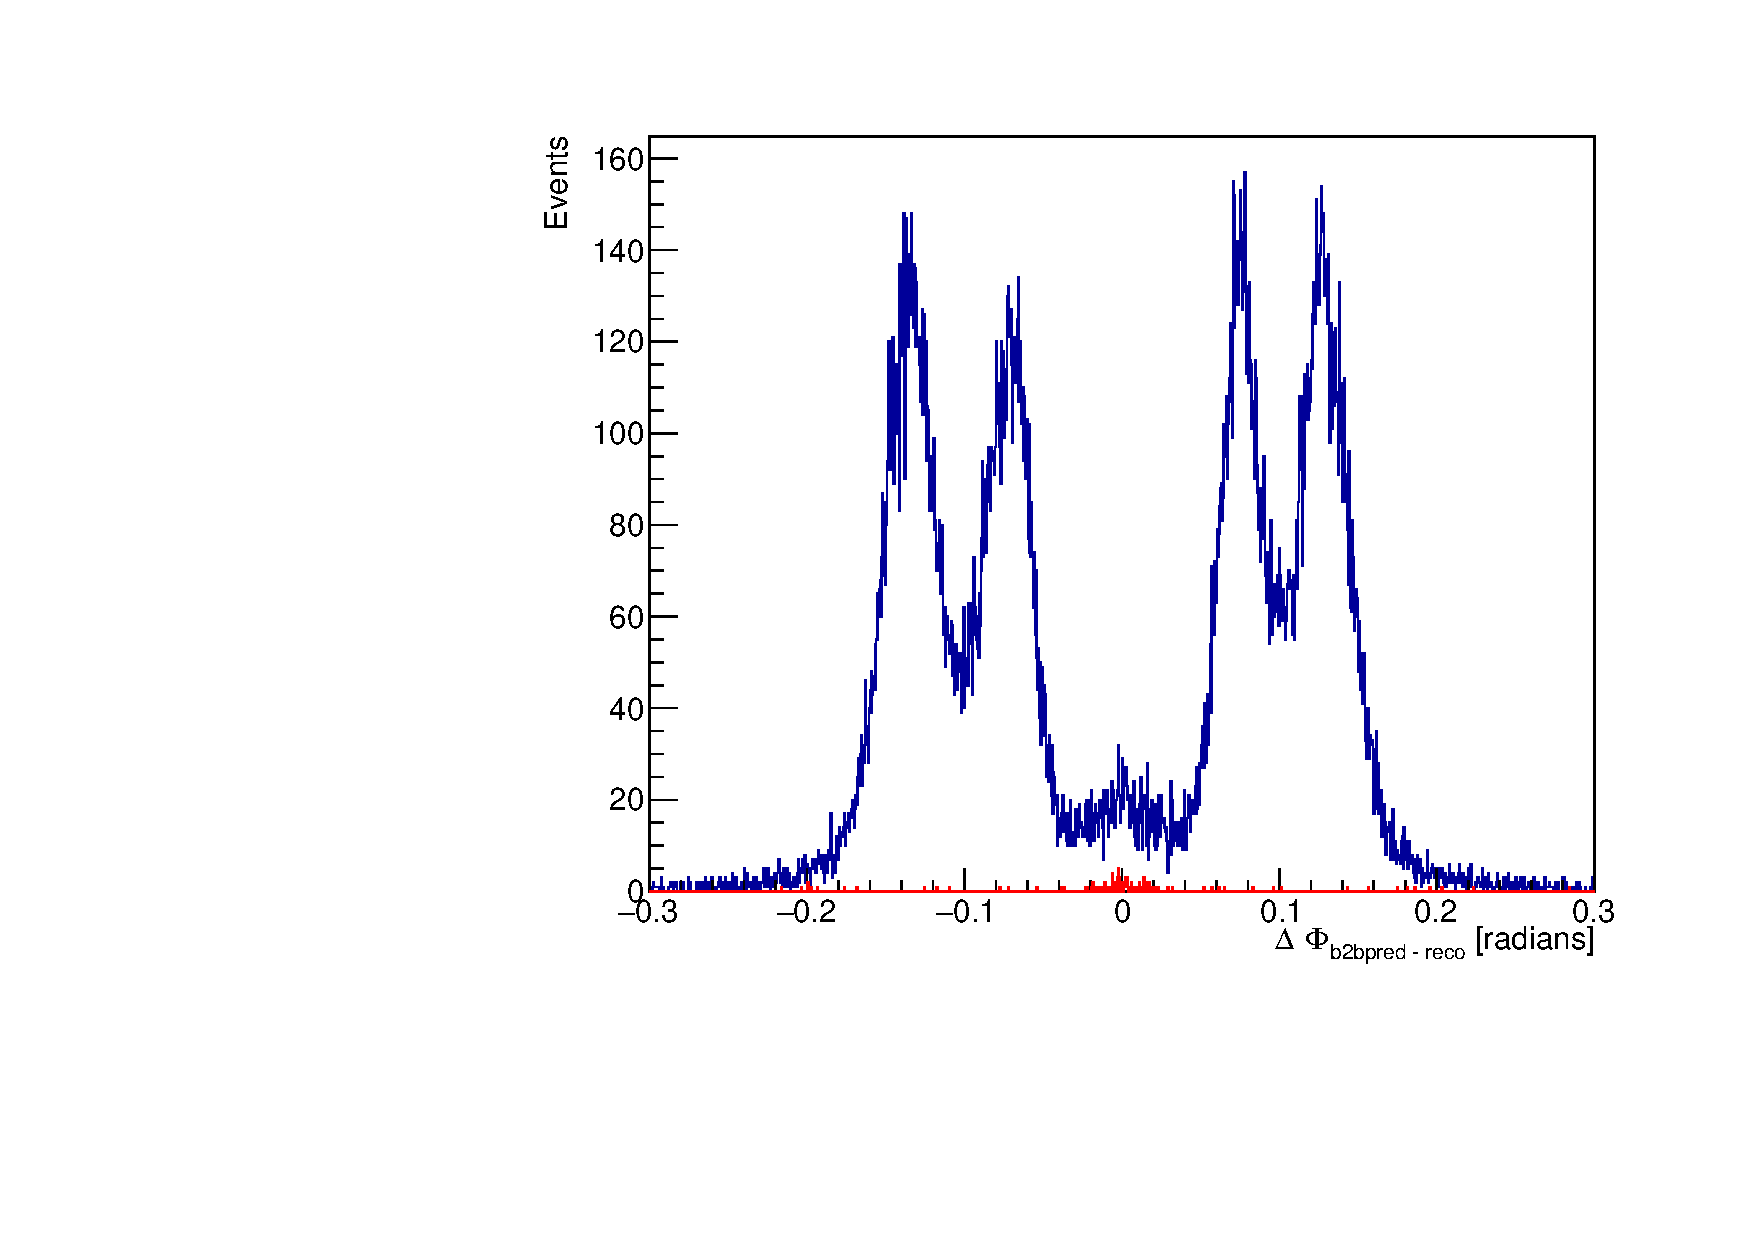
\includegraphics[width=4cm]{Plots/MCgg}
	\end{figure}
	
\end{textblock*}


\begin{textblock*}{\textwidth}(0cm,-0.5cm)
	\begin{figure}
		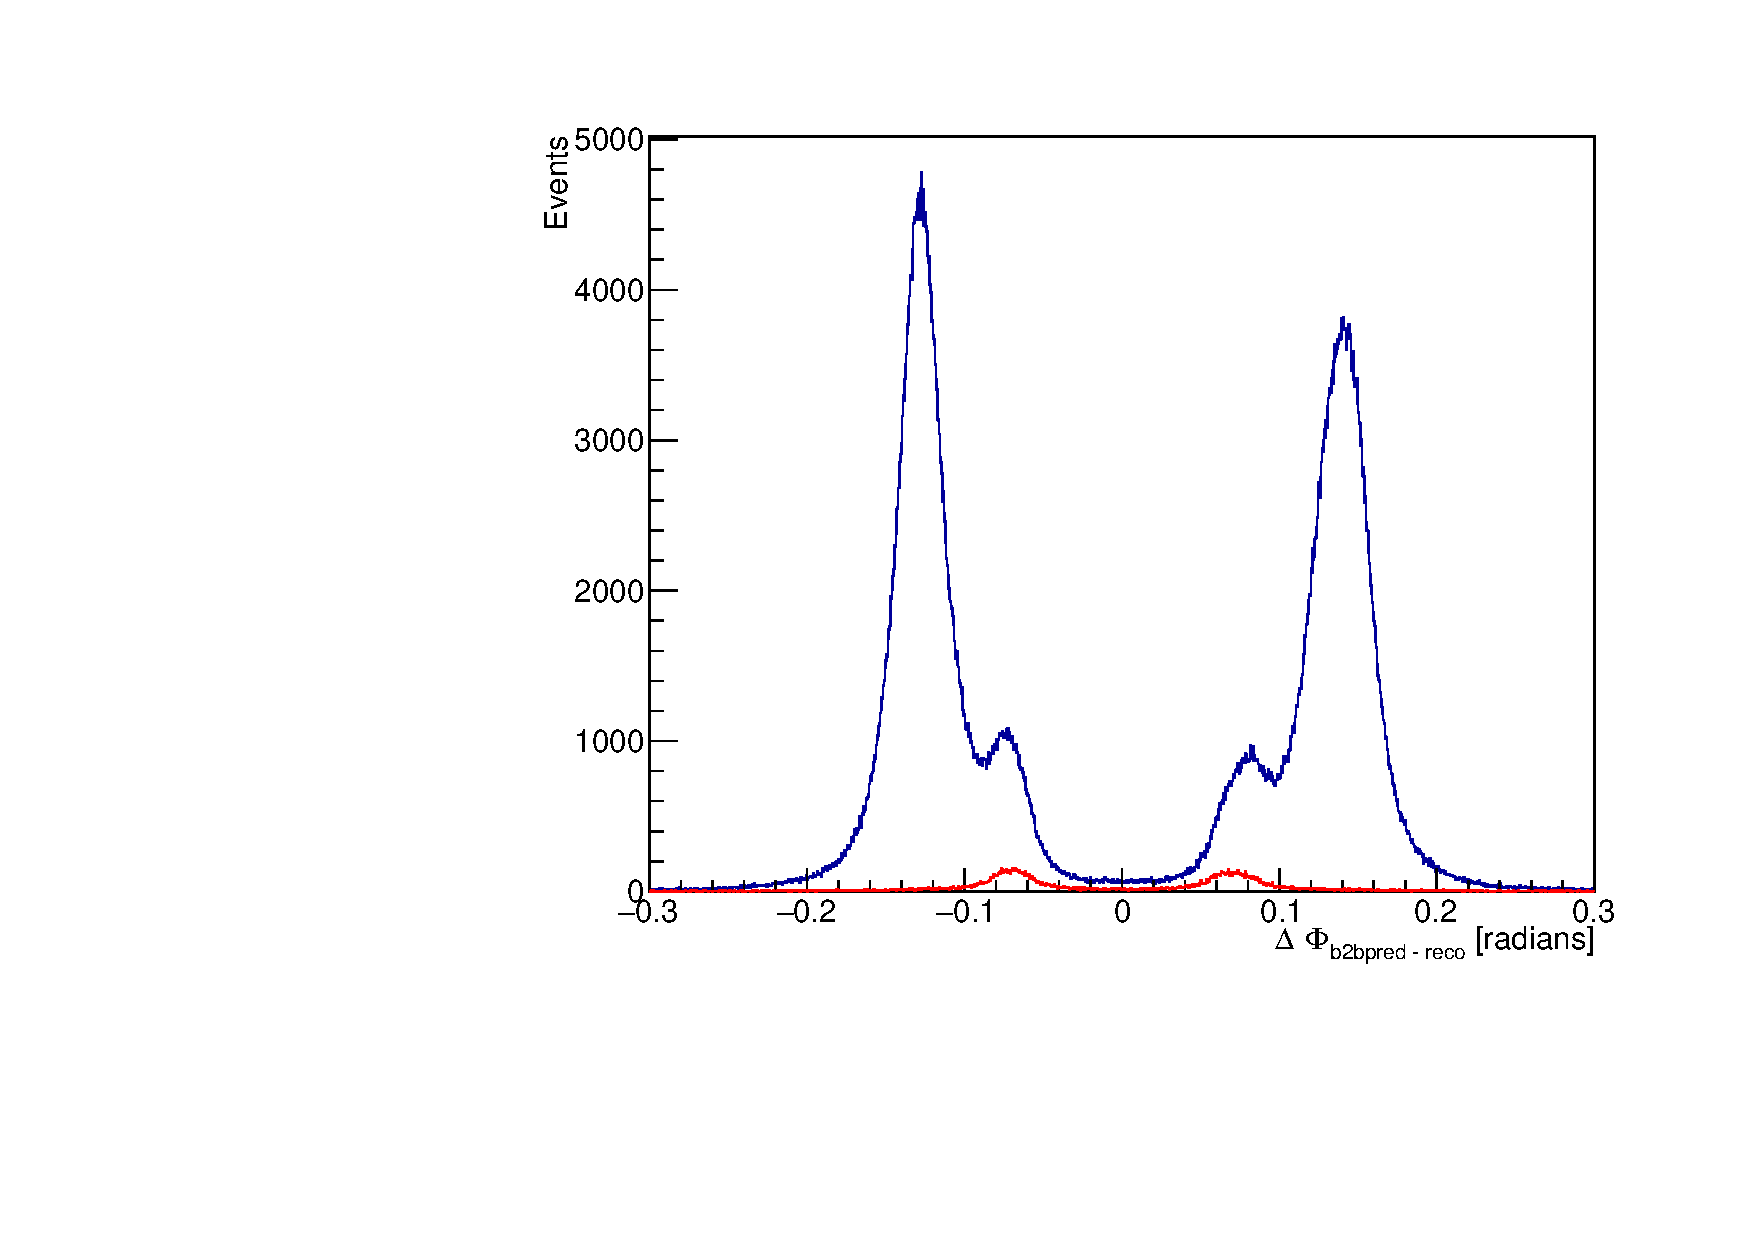
\includegraphics[width=4cm]{Plots/MCeg}
	\end{figure}
	
	\end{textblock*}	

\begin{textblock*}{\textwidth}(4cm,-0.5cm)
	\begin{figure}
		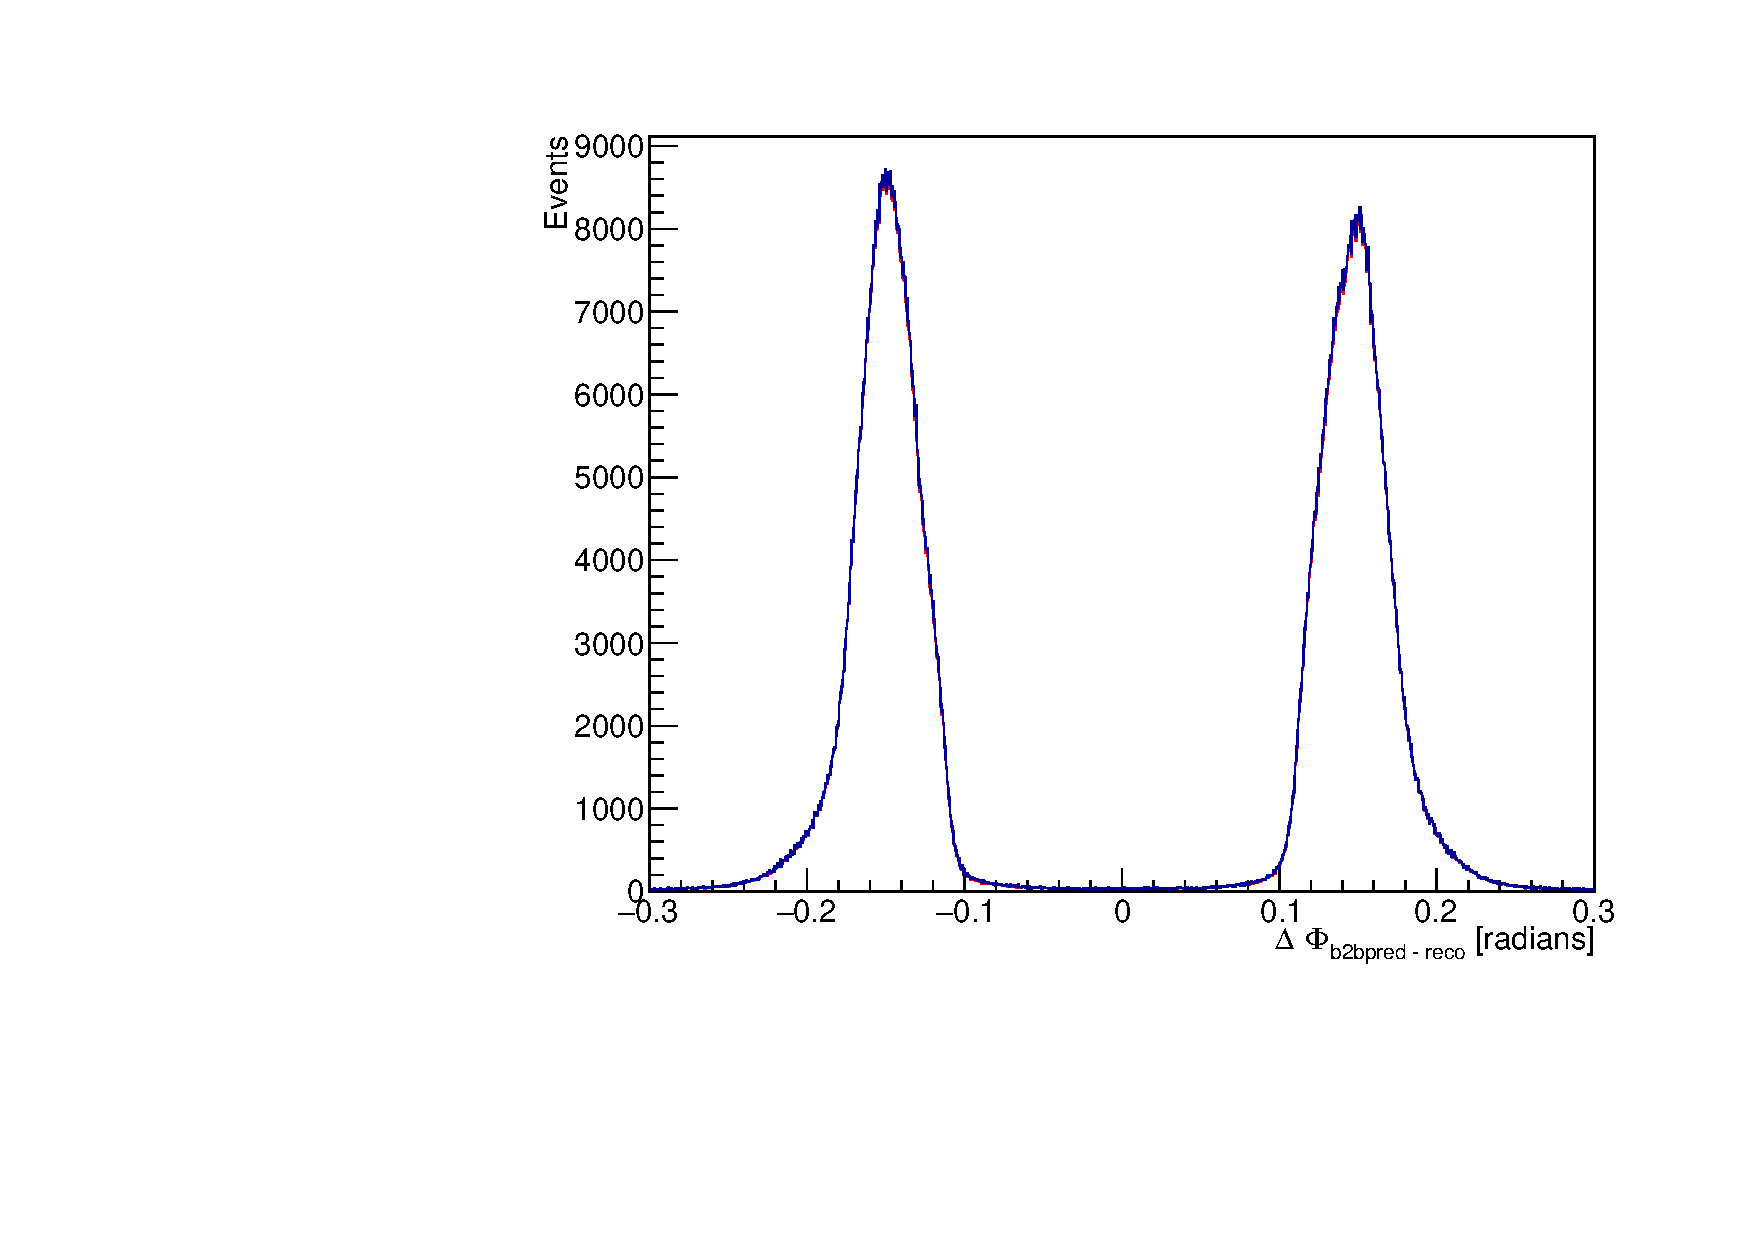
\includegraphics[width=4cm]{Plots/MCee}
	\end{figure}
	
\end{textblock*}	

\begin{textblock*}{\textwidth}(7.5cm,-3.35cm)
	\begin{itemize}
		\item MC11 $\textrm{ee} \rightarrow \textrm{ee}$ sample
		\item Reconstructed \textcolor{blue}{blue}
		\item MCTruthMatched \textcolor{red}{red}
	\end{itemize}
	
\end{textblock*}

\begin{textblock*}{0.2\textwidth}(0.0cm,3.3cm)
 Two clusters; No track
\end{textblock*}

\begin{textblock*}{0.2\textwidth}(4cm,3.3cm)
	Two clusters; One track
\end{textblock*}

\begin{textblock*}{0.2\textwidth}(8cm,3.3cm)
	Two clusters; Two tracks
\end{textblock*}


\begin{textblock*}{\textwidth}(5.2cm,-3.6cm)
	all
\end{textblock*}


\end{frame}



\begin{frame}{Multiple candidates}
	
	\begin{itemize}
		\item For some events, there is more than one vpho reconstructed
		\item One needs to select only one vpho per event
	\end{itemize}
	
	
	
		\begin{figure}
		\begin{subfigure}{.5\textwidth}
			\centering
			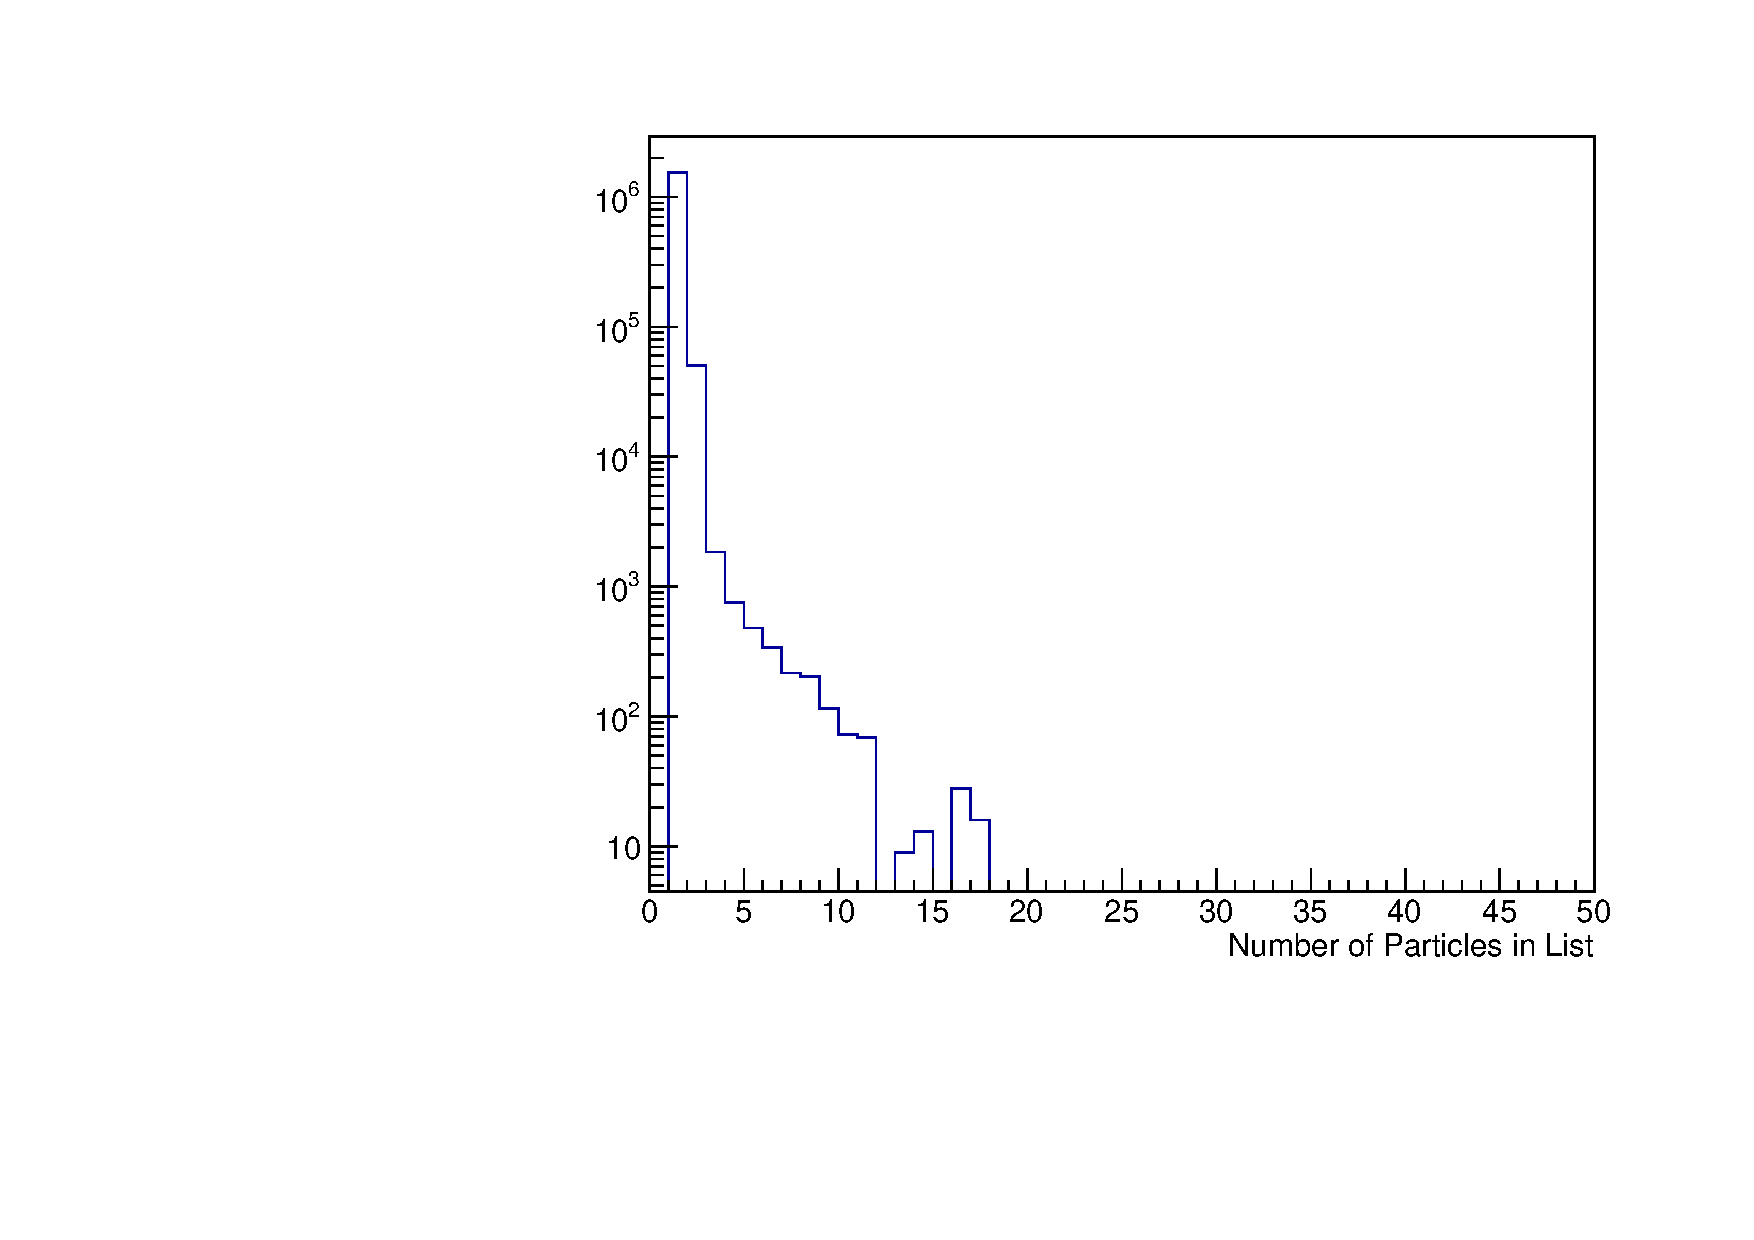
\includegraphics[width=4.5cm]{Plots/NumVpho}
			
			\label{fig:sub1}
		\end{subfigure}%
		\begin{subfigure}{.5\textwidth}
			\centering
			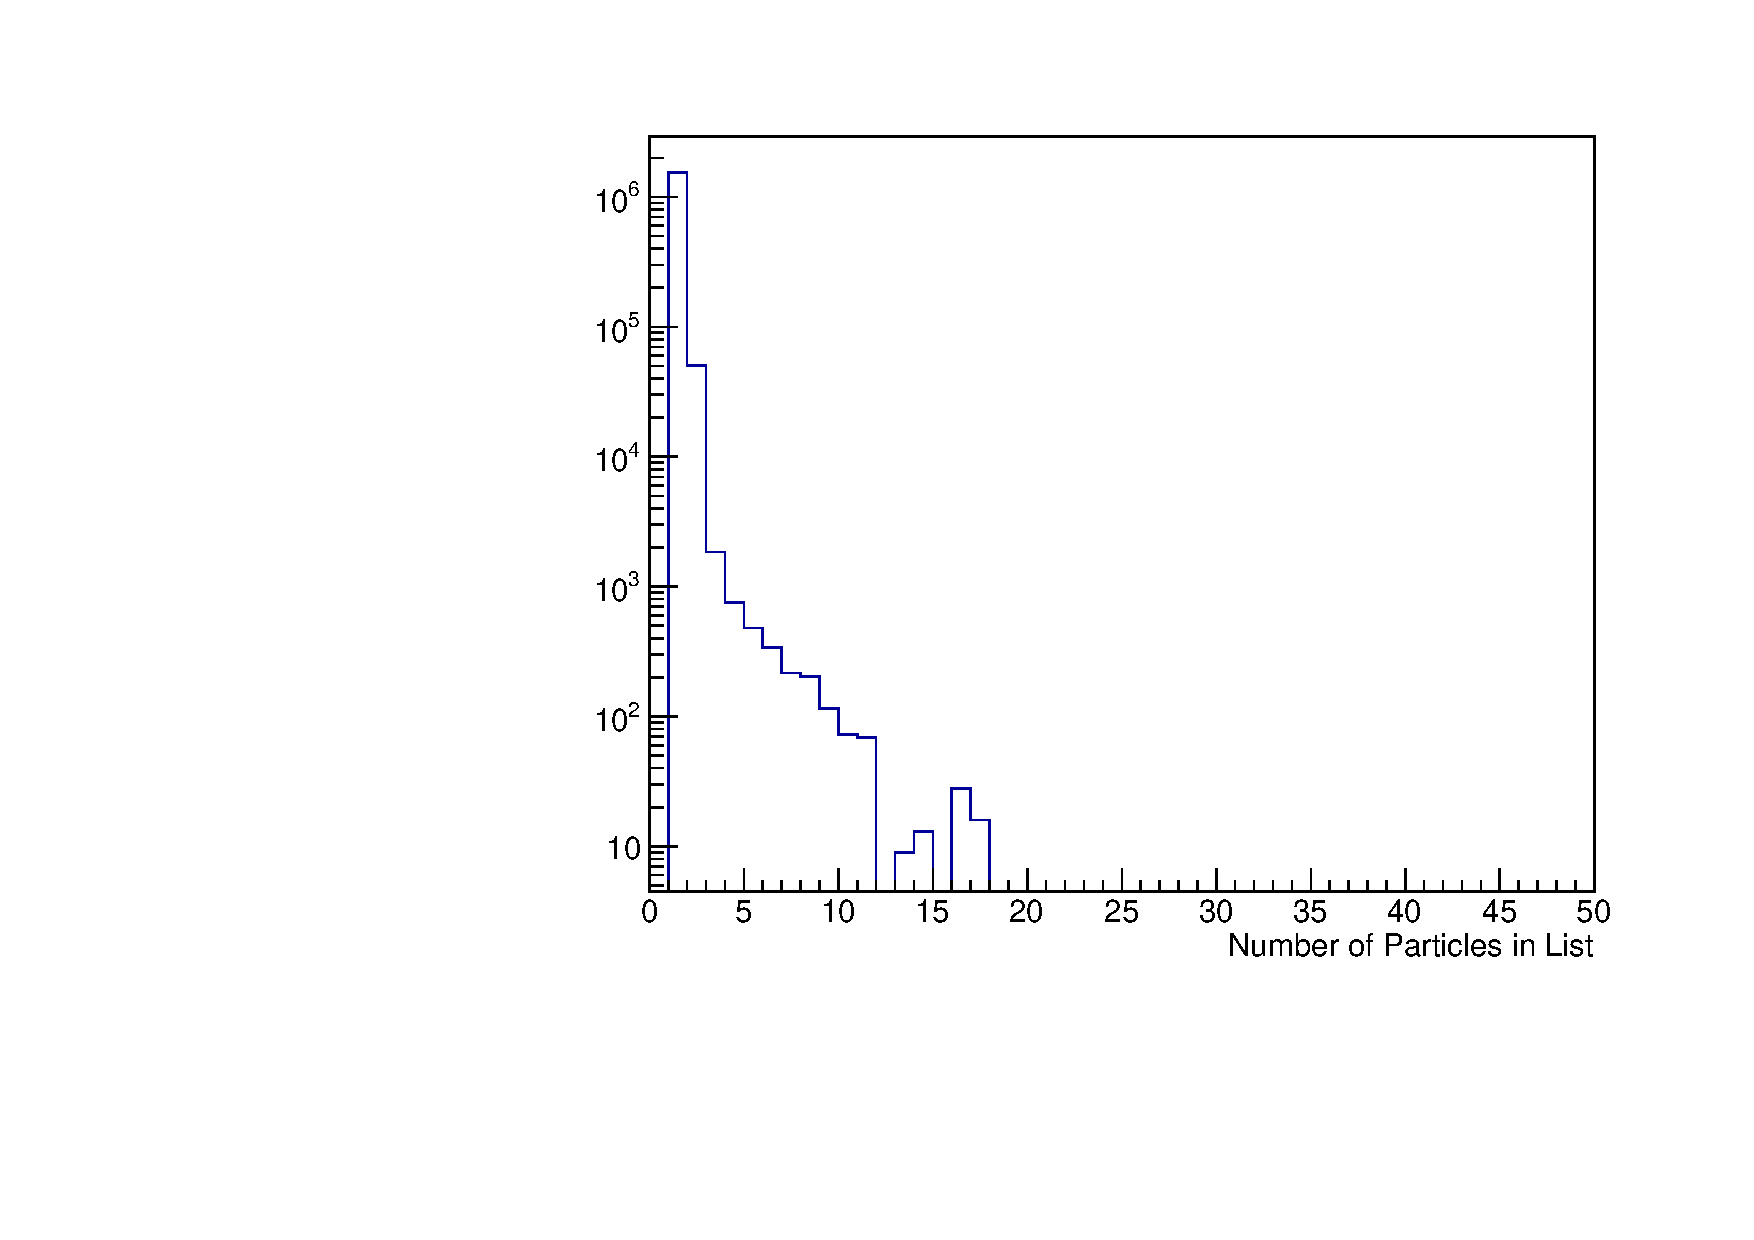
\includegraphics[width=4.5cm]{Plots/NumVphoMC}
			
			\label{fig:sub2}
		\end{subfigure}
		
		\label{fig:test}
	\end{figure}


\begin{textblock*}{\textwidth}(1.7cm,-4.2cm)
	Phase 2 Data
\end{textblock*}	


\begin{textblock*}{\textwidth}(7.8cm,-4.2cm)
	MC
\end{textblock*}

\begin{textblock*}{\textwidth}(6.7cm,-3.7cm)
	\begin{itemize}
	{\small	\item \textcolor{blue}{Reconstructed}}
	{\small	\item \textcolor{red}{MCTruthMatched}}
	\end{itemize}
\end{textblock*}
	
\end{frame}



\begin{frame}{Summary}
	\begin{itemize}
	\item After a rough beginning and a lot of gained experience, I am now (hopefully) on the right track 
	\item I hope to provide a first estimation shortly after Easter
	\item I still need to handle few things before it:
	\begin{itemize}
		\item Select the best $\textrm{vpho:bhabha}$ candidate
		\item Define the signal region in the $\Delta \Phi$ plot based on MC
	\end{itemize}
\end{itemize}
\end{frame}


\section{Collection}

\begin{frame}
Als erstes Sams plots nachmachen. Siehe andere Praesentation. Es geht um die triple Peaks und die 2D Delta Phi peaks. (andere presentation)
MassenCut von 8 ueberall.
Anschliessen ueber MC laufen. Man hat da alles besser unter kontrolle. Problem mit den Listen (siehe presentation).
MC muss erst komplett verstanden werden.
Es sollte eigentlich nur vpho pro event geben. $\rightarrow$ viel background. Erhoehe den MassCut von 8 auf 9 GeV. 

Es gibt auch einen Unterschied zwischen b2bPhi und b2bClusterPhi. bei b2bPhi wird noch beruecksichtigt um welches teilchenes sich gehandelt hat. Folglich wird auch die Krummung der Elektronen im Magnetfeld beruecksichtigt. Was wir aber wollen, um den nterschied zu bestimmen ist b2bphi. siehe skizze.
bei der skizze muss auch beachtete werden, dass eigentlich ins schwerpunktsystem geboostet wird dann der b2b angle bestimmt wird und dann wieder zurueck geboostet wird. das ist wichtig, weil der boost nicht genau entlang der x achse verlaeuft.
\end{frame}


\begin{frame}
	\begin{figure}
		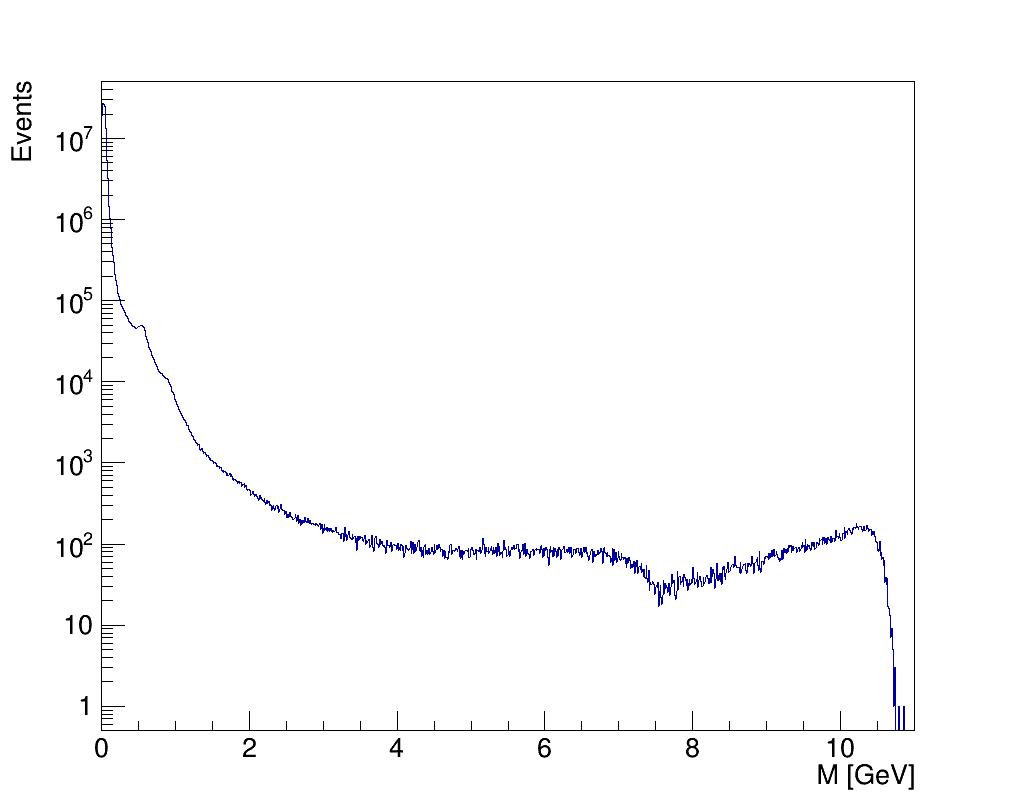
\includegraphics[width=6cm]{Collection/MCMNoCuts}
	\end{figure}
Masse des virtuellen Photons im Bhabha Event. Logarithmische Skala aufgrund des starken Backgrounds fuer kleine Massen. Als erstes wurde ein sehr grosszuegiger Cut mit M groesser als 8GeV gewaehlt um das Verhalten von MC besser zu verstehen.

\end{frame}




\begin{frame}
	\begin{figure}
		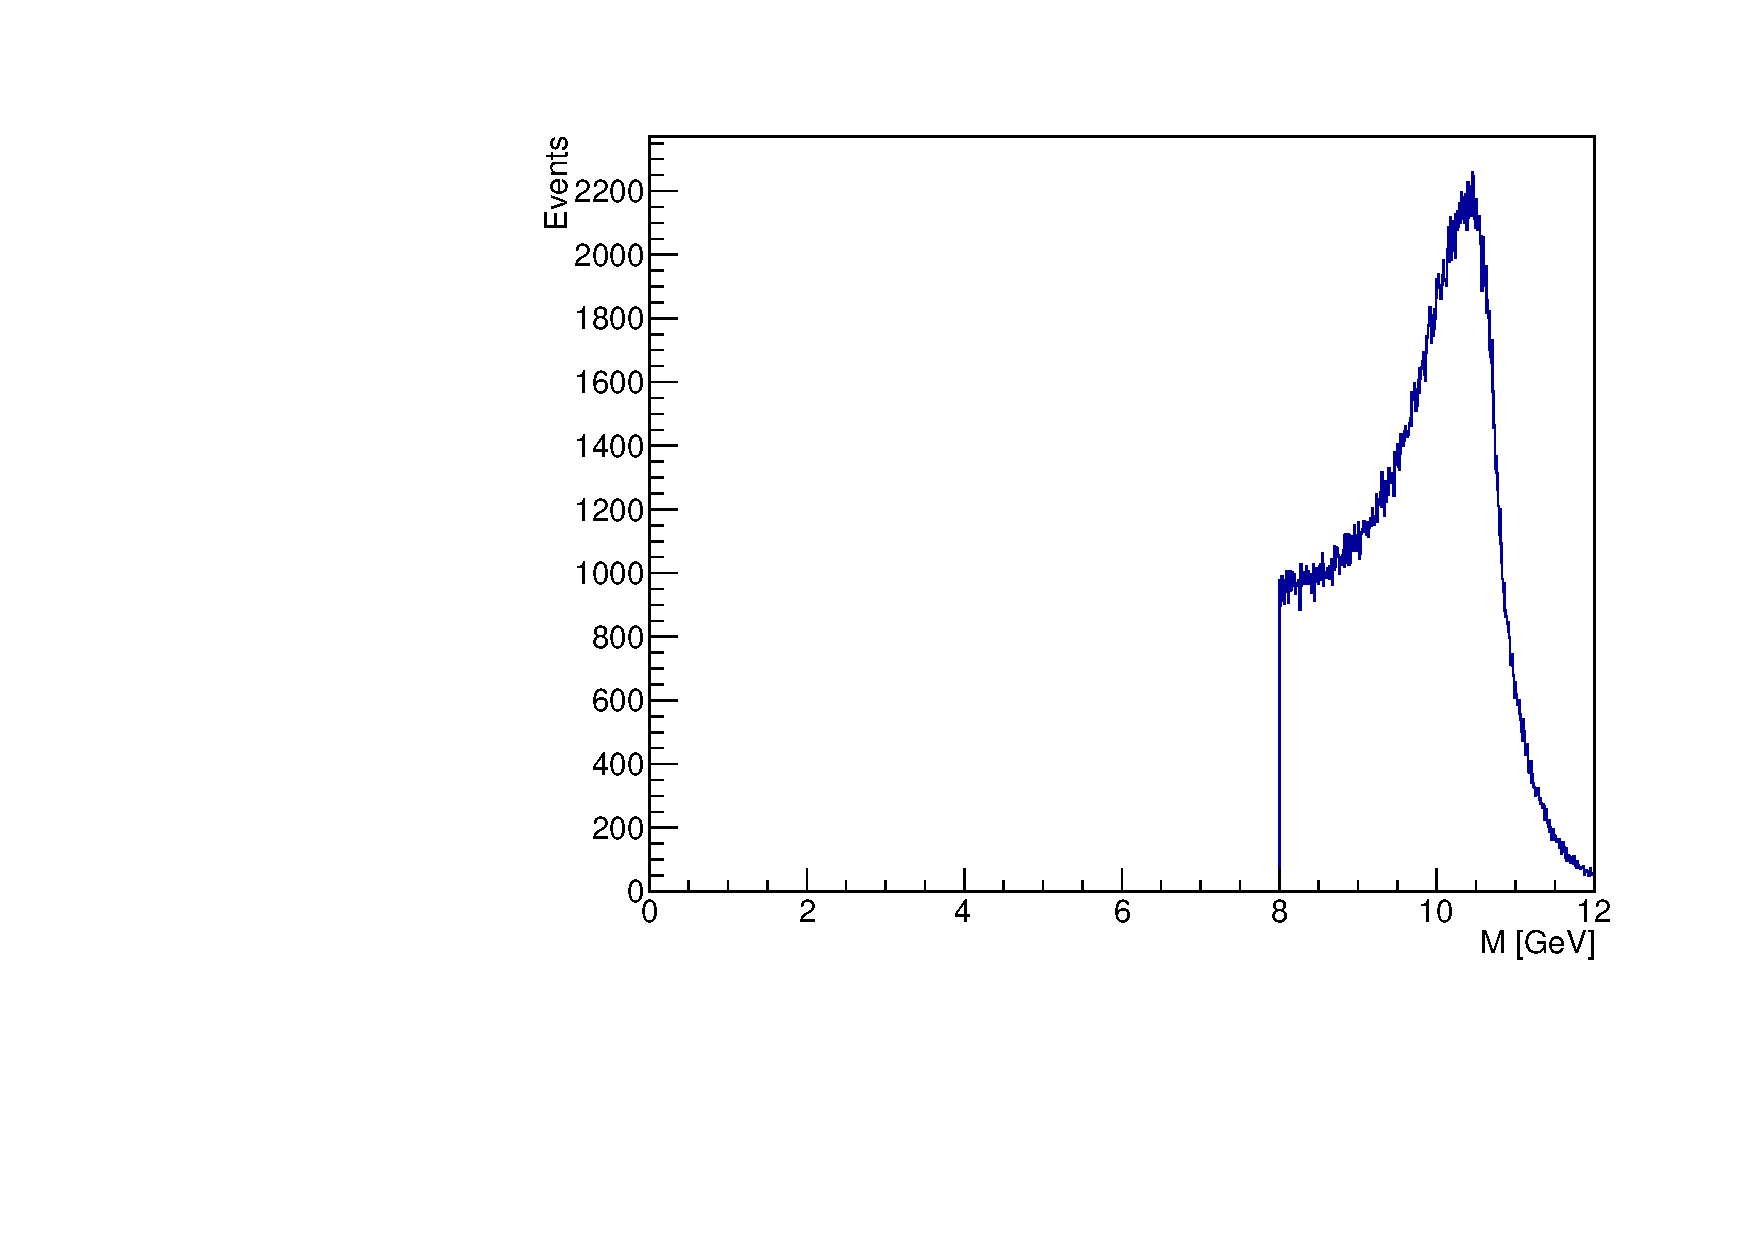
\includegraphics[width=6cm]{Collection/MCM8}
	\end{figure}

der erstmal einziger Cut der angewendet wird, um einen grossteil des backgrounds weg zu schneiden.

Zu sehen ist ausserdem der Peak bei M$\approx$ 10 GeV (\textit{invariante Masse}). Was der schwerpunktsenergie  des Beschleunigers entspricht. Man kann auch hier noch sehr viel Hintergrund vermuten.




\end{frame}





\begin{frame}
	\begin{figure} 
	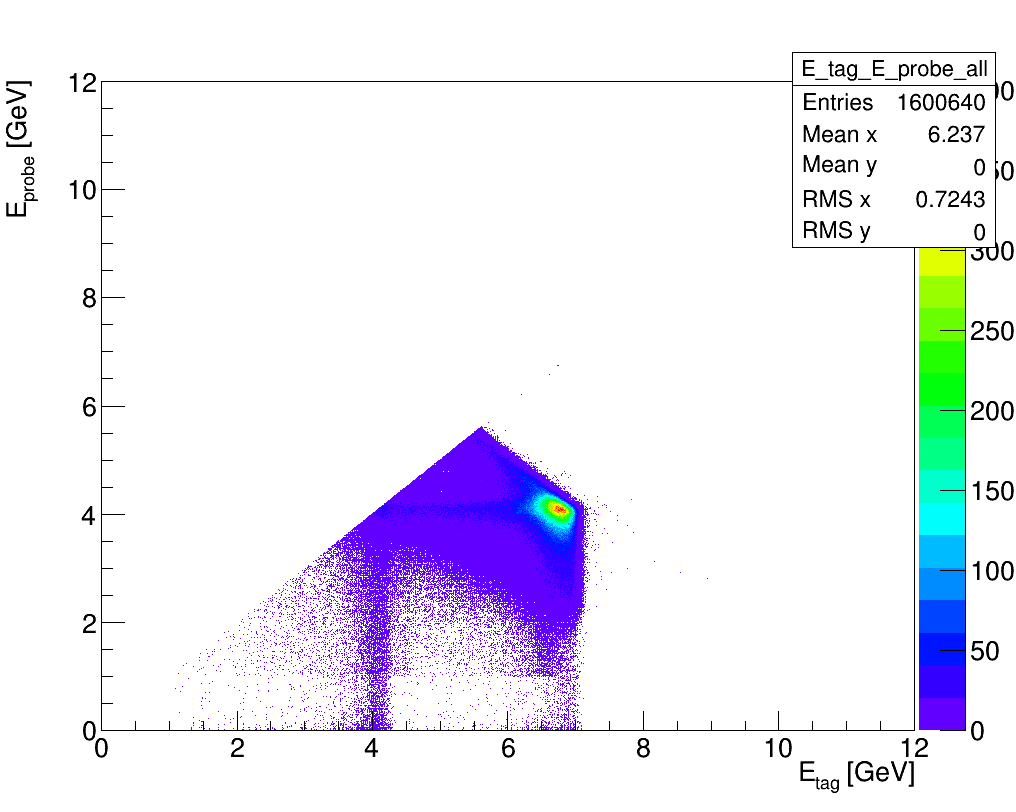
\includegraphics[width=6cm]{Collection/MCEE8_all}
\end{figure}

urspruenglich kein Cut auf die daughters damit man alles besser verstehen kann. In dem Plot sieht man dass ranking funkioniert. (kein Probe hat mehr energie als ein Tag) und dass ein cluster energy cut auf die daughters auch sinnvoll ist. auch beide daughters sollten auf clusterE gecutet werden. Dadurch wird automatisch verlangt dass sie den ECL treffen da nur dort cluster entstehen koennen. Ein theta cut wird dadurch nicht mehr benoetigt
. 


\end{frame}

\begin{frame}

	\begin{figure}
		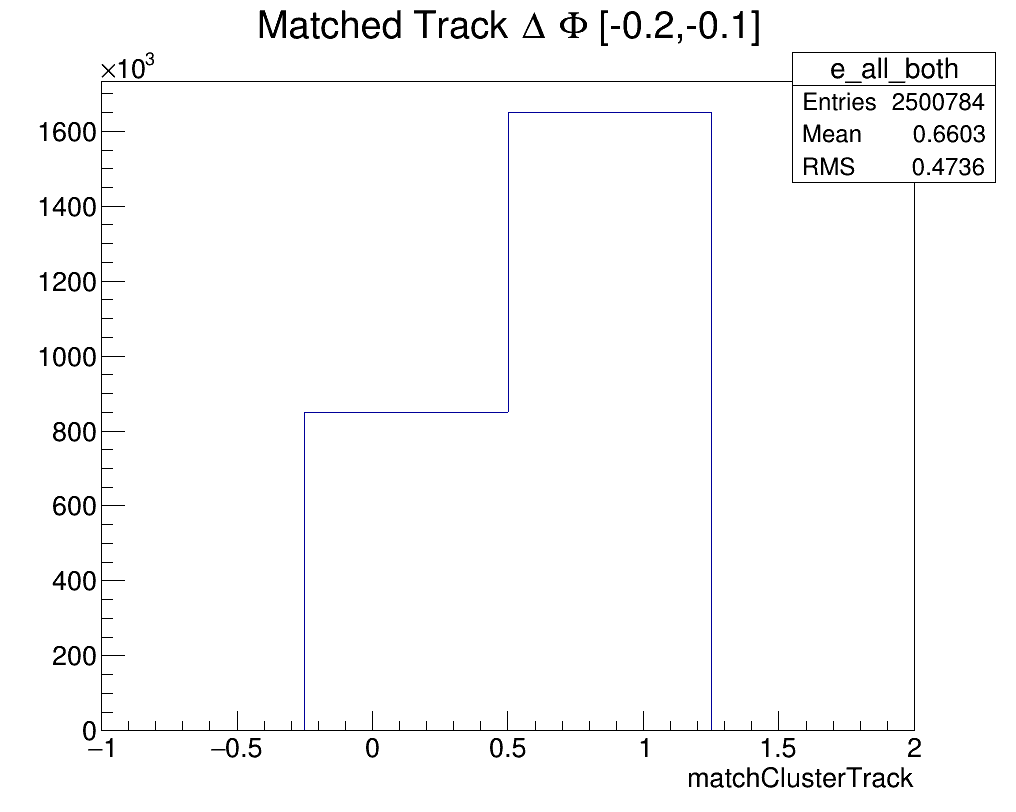
\includegraphics[width=3cm]{Collection/firstEffMC8NoEE}
	\end{figure}

erste efficiency auf MC. Events mit 2 tracks und 2 cluster rechts und events mit 2 cluster und 1 tracks links. Plot vor nCandsCut (also noch viele nCands vpho pro event) plot vor energy und time cut auf die daughters. pi mal daumen ist das eine efficienz von nur rund 70prozent und das waere fatal $\rightarrow$ hoffentlich ist das meiste durch background verursacht und wird besser mit den weiteren cuts . (sollte wirklich nicht sein). es wurde auf die triple delta phi plots geschnitten. Es wurde sich auf den rechten konzentriert $\rightarrow$ $"( daughter\_0\_b2bClusterPhi - daughter\_1\_clusterPhi) > -0.2 \&\& (daughter\_0\_b2bClusterPhi - daughter\_1\_clusterPhi) < -0.1 \&\& M>8.0"$

Hier wurde doppelt gezaehlt. Sollte aber bei der Effizienz nicht so schlimm sein(oder?) 


\end{frame}

\begin{frame}

\begin{figure}
	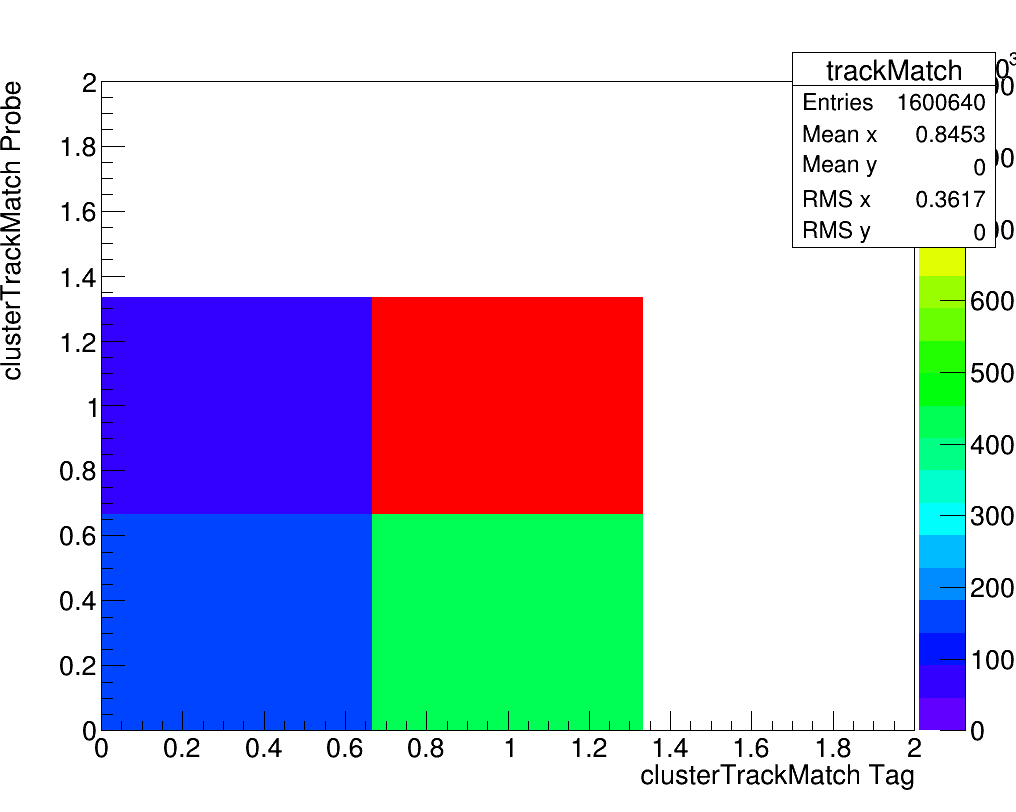
\includegraphics[width=3cm]{Collection/MCtrackMatch8}
\end{figure}
immer noch vor energy timing nCand vpho Cuts. es geht hier darum wenn duahgter 1 einen track hat, hat daughter 0 dann auch einen und anders herum. Meistens haben beide einen Track (gut das ist effizienz). Das naechst haeuffigste ist dass beide keinen Track besitzen. Davon gibt es mehr Eintraege als das Probe einen Track hat und Tag nicht. (Pures bhabha sample).


\end{frame}

\begin{frame}
	\begin{figure}
		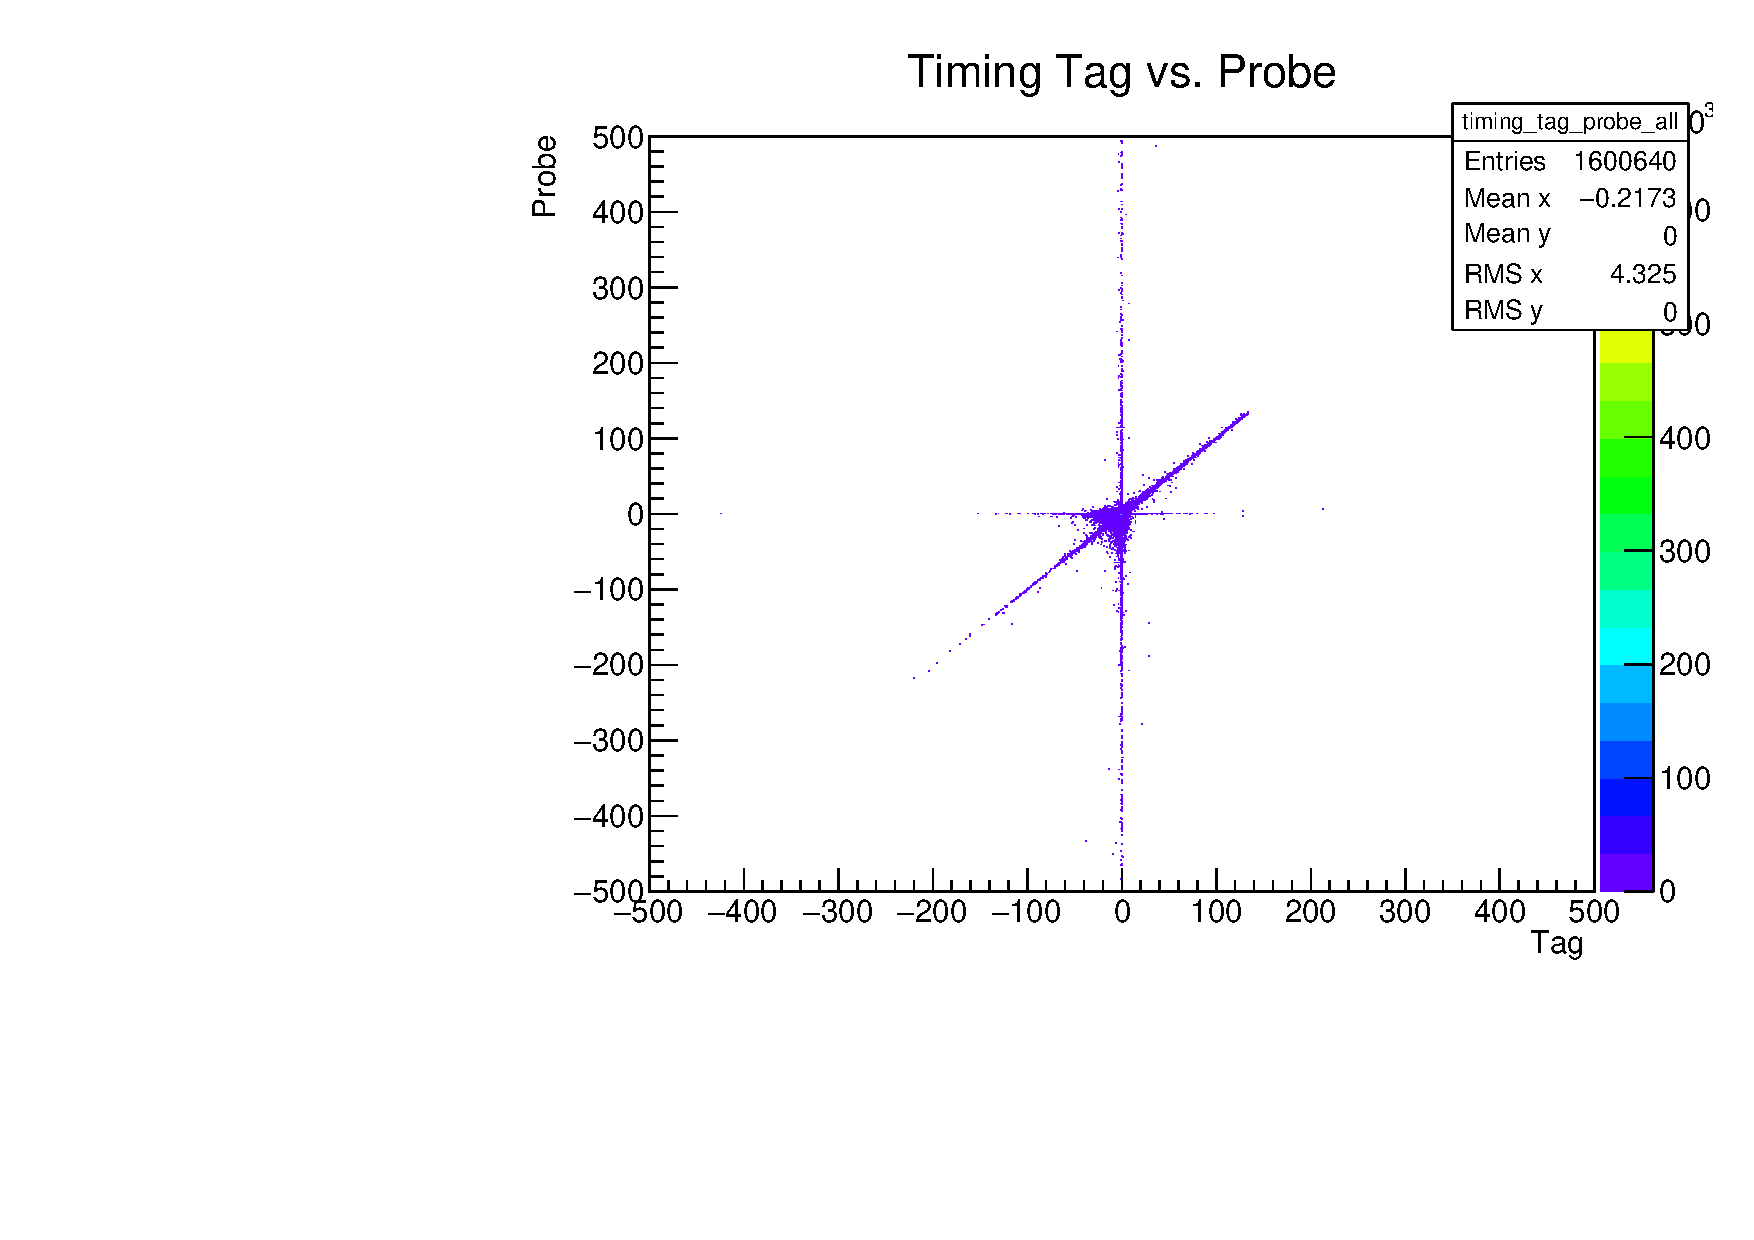
\includegraphics[width=6cm]{Collection/MCclusterTiming8}
	\end{figure}

clusterTiming fuer probe und tag. in [ns?] komische struktur. Wieder vor allen energy timing nCand vpho Cuts.  M(vpho) groesser als 9GeV. Diagonale kommt mir komisch vor. Ich nehme mal an, dass die events an denen ich interessiert bin, sich um die 0,0 befinden. Bzw auf der diagonalen, denn dann haben wir eine Korrelation zwischen den beiden daughters


\end{frame}

\section{Verbesserung der Cuts}

\begin{frame}
	Es muessen eindeutig Cuts eingefuehrt, bzw verbessert werden.
	
	Deswegen erstmal den MassenCut erhoehen. Einen EnergieCut auf die daughters einfuehren. Cuts aufs Timing.
	
	Theta Winkel von Tag muesste eigentlich immer kleiner sein als der von tag. Auch sollte Tag eigentlich keinen Theta Winkel von 90 Grad oder mehr besitzen.
	
	Und dann nochmal nCands plotten und hoffen, dass es deutlich runter geht.
	
	Erstmal MC deutlich besser verstehen
	
	
	
	
	
	
\end{frame}




\end{document}
